\section{Аналитическая часть}

\subsection{Формализация задачи}
В данной курсовой работе будут использоваться следующие понятия: запись времени, тег, проект, цель.

Запись времени -- это временной интервал, содержащий название деятельности, которой занимался человек в течении этого интервала.

Тег -- это метка, присваиваемая к объекту записи. Теги используются для категоризации, организации и быстрого поиска информации. В контексте онлайн трекера времени теги могут использоваться для классификации записей времени по проектам, клиентам или задачам.

Проект -- специальная метка, относящая запись времени к определенной повторяющейся деятельности, например "спорт"\ или "курсовой проект".

Пример  структуры записи:
\begin{itemize}[leftmargin=1.6\parindent]
	\item "13:00 - 14:00 | 1 час"\  -- интервал;
	\item "аналитическая часть"\ -- название деятельности;
	\item "курсовой проект"\ -- проект;
	\item "за компьютером"\ -- тег.
\end{itemize}

Цель -- временной интервал, в течении которого нужно потратить заданное количество часов на определенный проект. Пример цели -- с 1.09.2023 по 9.09.2023 потратить на проект "Курсовая работа"\ 10 часов.

\newpage
Возможности пользователя:
\begin{itemize}[leftmargin=1.6\parindent]
	\item создание проекта;
	\item создание записи;
	\item создание тега;
	\item составление целей;
	\item добавление других пользователей в друзья;
	\item отслеживание временных затрат за определенный период пользователя и его друзей;
	\item отслеживание выполнения целей.
\end{itemize}

\newpage

На рисунке \ref{fig:usecase} представлена диаграмма использования приложения.
\begin{figure}[hbtp]
	\centering
	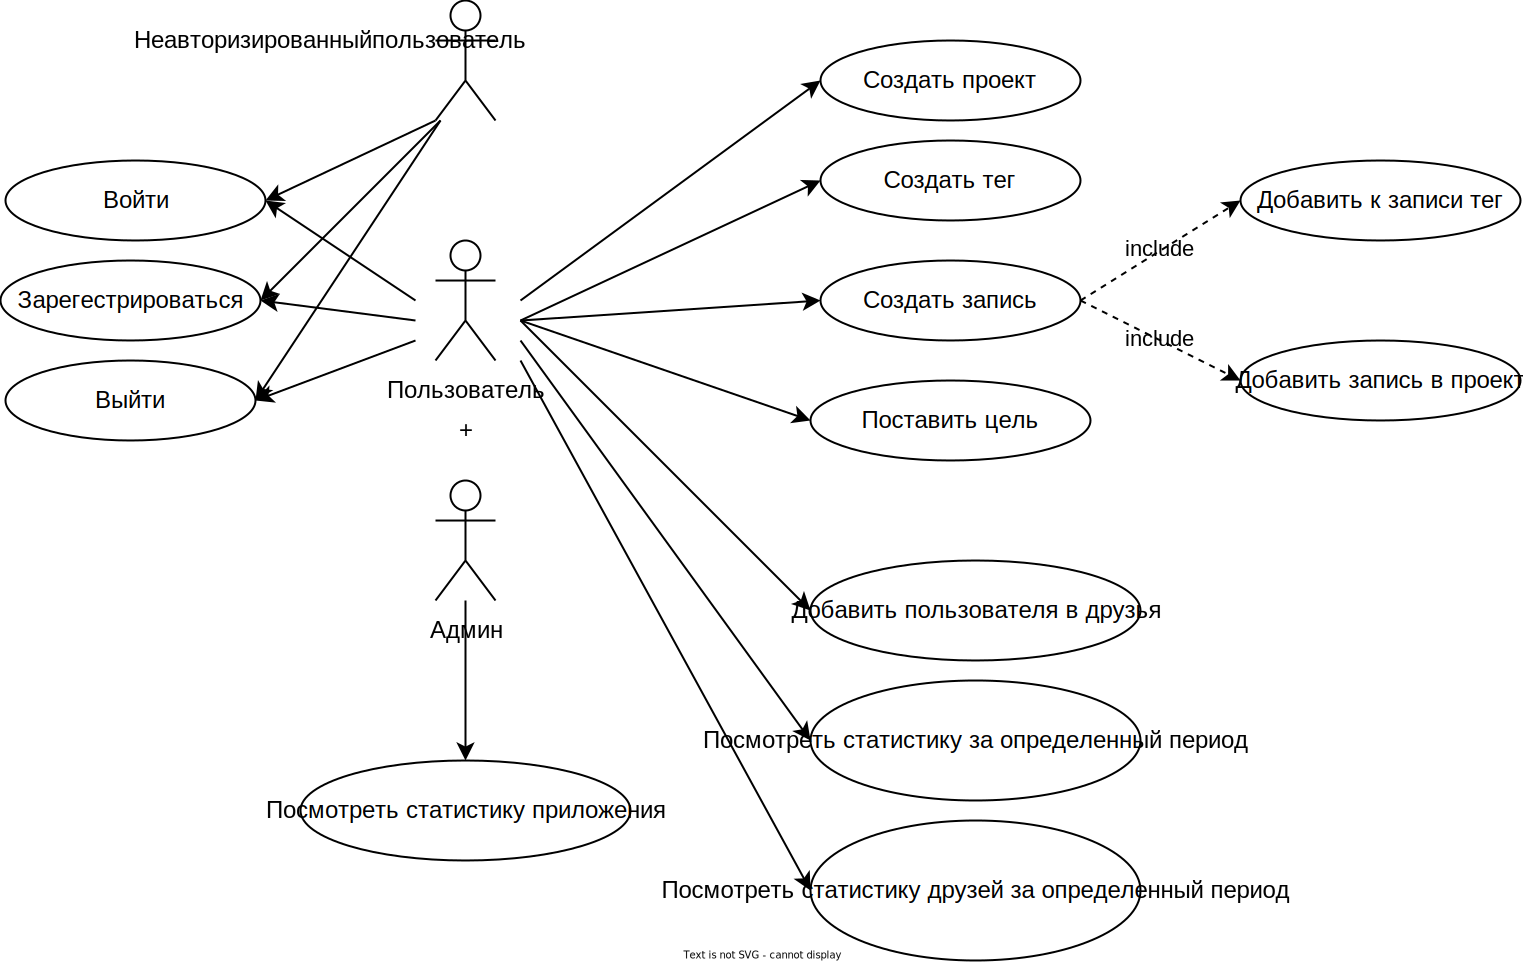
\includegraphics[width=\textwidth]{img/Usecase.drawio.pdf}
	\caption{Диаграмма использования приложения}
	\label{fig:usecase}
\end{figure}

\subsection{Пользователи и данные в системе}

Система, разрабатываемая в рамках курсового проекта, предполагает собой REST-API веб сервис \cite{rest-api}.

Доступ к системе имеет разграничение по ролям: неавторизированный пользователь, авторизированный пользователь и администратор. При этом\\ должно быть ограничение доступа к данным в зависимости от роли пользователя.

\newpage
Функционал каждой роли представлен в таблице \ref{tbl:role}.

\begin{table}[h]
	\centering
	\caption{Типы пользователей и их функционал}
	\label{tbl:role}
	\begin{tabular}{|l|p{9cm}|}
		\hline
		\textbf{Тип пользователя} &\textbf{Функционал} \\
		\hline
		Неавторизованный пользователь & Регистрация, авторизация \\
		\hline
		Авторизованный пользователь & Создание проекта, тега, записи, цели, добавление в друзья, просмотр статистики друзей, отслеживание выполнения целей \\
		\hline
		Администратор & Весь функционал авторизированного пользователя, просмотр данных каждого пользователя без добавления в друзья, просмотр статистики приложения(сколько пользователей, проектов, целей)\\
		\hline
	\end{tabular}
\end{table}

Данные в приложении можно разделить на несколько типов:

\begin{itemize}[leftmargin=1.6\parindent]
	\item сессии;
	\item данные о пользователях;
	\item записи времени;
	\item проекты;
	\item теги;
	\item связи между пользователями;
	\item цели.
\end{itemize}

\newpage
\subsection{Модели данных}

Модель данных --  это абстрактное, самодостаточное, логическое
определение объектов, операторов и прочих элементов, в совокупности
составляющих абстрактную машину доступа к данным, с которой
взаимодействует пользователь. Эти объекты позволяют моделировать
структуру данных, а операторы — поведение данных\cite{db}.

Существует 4 основных типа моделей организации данных:

\begin{itemize}[leftmargin=1.6\parindent]
	\item иерархическая;
	\item сетевая;
	\item реляционная;
	\item нереляционная.
\end{itemize}

\subsubsection{Иерархическая модель}

В иерархической модели данных используется представление базы данных
в виде древовидной структуры, состоящей из объектов разных уровней. Среди
объектов существуют связи, любой объект может включать в себя нес\-колько
объектов более низкого уровня. Такие объекты находятся в отношении предка к
потомку, при этом вероятна ситуация, когда объект-предок имеет нес\-колько
потомков, тогда как у объекта-потомка обязательно должен быть только один
предок.

Основной недостаток иерархической модели данных заключается в ее ограничении на строго иерархические отношения между элементами что приводит к тому, что невозможно реализовать отношение "многие ко многим "\ .
\subsubsection{Сетевая модель}

Сетевая модель -- это структура, у которой любой элемент может быть связан
с любым другим элементом.

Сетевые базы данных, являются своеобразной модификацией иерархических баз данных. Отличаются от иерархических лишь тем, что у дочернего элемента может быть несколько предков, то есть, элементов стоящих выше него. 

Достоинством сетевой модели данных является ее быстродействие в отличие от иерархической БД, гибкость в хранении данных, универсальность в сравнении с другими моделями, а также возможность доступа к данным через значения нескольких отношений.

Основным недостатком является то, что сетевая модель не поддерживает простого доступа к данным, так как для доступа к определенной записи необходимо проходить через несколько уровней связи, что затрудняет работу с данными и усложняет их поддержку и модификацию. 

\subsubsection{Реляционная модель}
Реляционная модель данных является совокупностью данных и состоит из
набора двумерных таблиц. При табличной организации отсутствует
иерархия элементов. Таблицы состоят из строк -- записей и столбцов -- полей.
На пересечении строк и столбцов находятся конкретные значения. Для каждого
поля определяется множество его значений. За счет возможности просмотра
строк и столбцов в любом порядке достигается гибкость выбора подмножества
элементов.

Взаимодействие с реляционными базами данных осуществляется с помощью SQL (Structured Query Language)\cite{sql}, стандартизированного языка запросов данных.

Работа с реляционными базами данных базируется на понятии внешних ключей, которые обеспечивают связь между таблицами. Внешний ключ является связующим элементом, который ссылается на первичный ключ другой таблицы и позволяет объединять данные из разных таблиц в один запрос.

Оптимизация работы с базами данных основывается на использовании индексов. Индексы позволяют ускорить поиск данных в таблице. Учитывая большой объем данных, применение индексов позволяет значительно ускорить процесс запроса значений.

Основным преимуществом реляционных баз данных является их интуитивная понятность и удобство использования, так как они основаны на простых концепциях, что упрощает группировку, фильтрацию и агрегацию данных.

\subsubsection{Нереляционная модель}
Данные нереляционных баз данных не имеют общего формата, в них для хранения используется не система из строк и столбцов, а применяется модель, которая оптимизирована для хранения определённого типа содержимого. Например, данные могут храниться в виде документов JSON \cite{json}, графов, а также пар ключ-значение.

Преимущества модели - возможность создания сложных структур данных, удобство при работе с объектами. Недостатки - сложность реализации, неудобство при работе с большим количеством данных.

\subsubsection{Выбор модели базы данных для решения задачи}

Для решения задачи будет использоваться реляционная модель данных
по описанным причинам:

\begin{itemize}[leftmargin=1.6\parindent]
	\item известна структура данных, которая редко меняется;
	\item структура данных не является сложной(с вложенностью, древовидной);
	\item наличие стандартизированного высокоуровневого языка запросов SQL.
\end{itemize}

Для хранения сессий пользователей следует использовать нереляционную модель, так как у сессий нет отношений и связей, они хранятся парами "key-value"\ .

В качестве решения задачи хранения сессий зачастую используются in-memory СУБД.

In-Memory СУБД -- это система, которая хранит данные в оперативной памяти компьютера. Это позволяет обеспечить высокую скорость доступа к данным и выполнения запросов, поскольку не требуется считывание и запись данных на диск. 

Такие СУБД относятся к нереляционным. 

\subsection{Формализация данных}
\subsubsection*{База данных пользователей, записей времени, проектов, тегов, целей  и отношений между ними}
Данные пользователей, записей времени, проектов, тегов, целей  и отношений между ними должны храниться в одной базе данных, так как данные связаны между собой.

На рисунке \ref{fig:ER} представлена ER-диаграмма в нотации Чена.


\begin{figure}[hbtp]
	\centering
	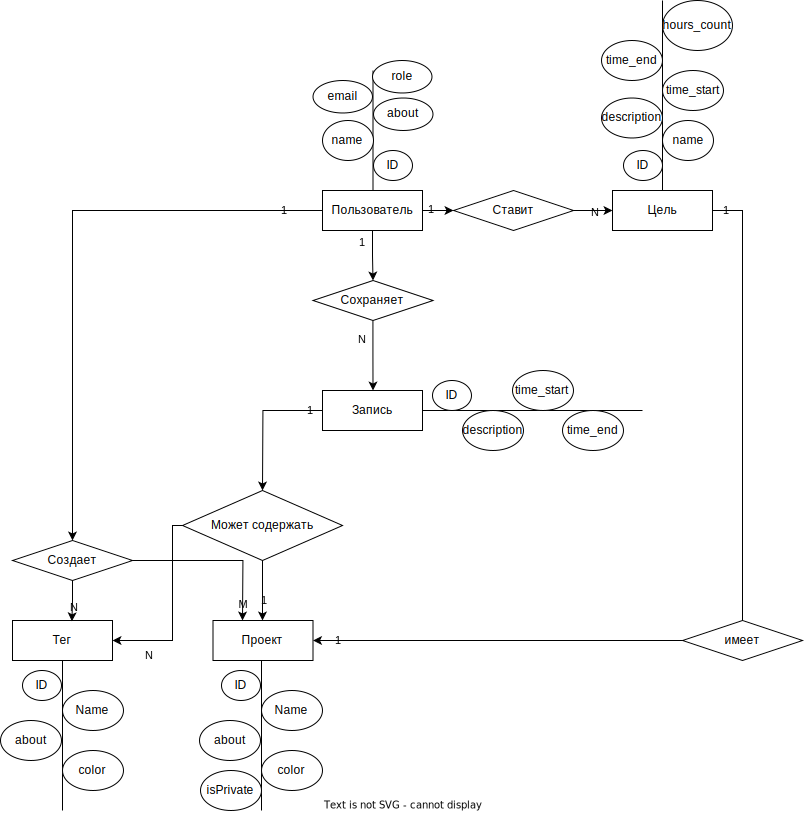
\includegraphics[width=\textwidth]{img/ER.drawio.pdf}
	\caption{ER-диаграмма сущностей}
	\label{fig:ER}
\end{figure}

\subsubsection*{База данных сессий} \label{5000}

Современные веб-приложения работают на основе HTTP протокола, который не хранит свое состояние, то есть каждый запрос обрабатывается как отдельная транзакция. Чтобы избежать необходимости повторной аутентификации пользователя при каждом запросе, необходимо самостоятельно отслеживать взаимодействие клиентов с приложением. Для этого используются сес\-сии\cite{sessions}, которые хранят "состояние"\ между сайтом и клиентом. 

Для эффективного хранения данных сессий, необходимо использовать специальную базу данных, в которой хранятся уникальные идентификаторы пользователей и сессий. Также необходимо обеспечить быстрое получение данных и защиту от сбоев системы, например, сохранять данные на диск с возможностью восстановления.

\subsection*{Вывод}
В данном разделе:

\begin{itemize}[leftmargin=1.6\parindent]
	\item формализована задача;
	\item определены и описаны роли доступа к  данным приложения;
	\item определены типы данных приложения;
	\item приведена диаграмма использования приложения;
	\item проанализированы и выбраны модели данных;
	\item формализованны данные, используемые в системе.
\end{itemize}



\pagebreak